\chapter{Literature Review}

In this chapter, we will look at some related research papers. These research papers guide us to choose a set of software quality metrics, quantify software quality attributes, and provide an important framework to build SQAT. We will also examine an open source tool and a commercial tool to gain more insights on the way we build SQAT. 

\section{Academic Research}

Software quality metric measures some properties of a software system \cite[]{washizaki2007framework}. By measuring software quality metrics, we can evaluate software development process, receive earlier feedback during the development, and assess the progress of software development \cite[]{yi1994goal}. By having SQAT in School of Computer Engineering, students can develop better codes and professors can evaluate programming assignments in a comprehensive way. 

Many software quality metrics have been defined in various researches. \cite{de2015classifying} has classified 570 software quality metrics related to maintainability in Metric Catalog System \footnote{Metric Catalog System can be accesses at http://julianasaraiva.info/oosmMetricsPortal}. However, previous works have shown that many software quality metrics are lacking a theoretical basis \cite[]{vessey1984research} or being too labor-intensive to collect \cite[]{kemerer1993reliability}. To avoid these problems \cite{chidamber1994metrics} has listed six design metrics with theoretical base, i.e. weighted methods per class, depth of inheritance tree, number of children, coupling between object classes, response for a class, and lack of cohesion in methods. \cite{harrison1998evaluation} also listed six valid Metrics for Object-Oriented Design (MOOD), i.e. method hiding factor, attribute hiding factor, method inheritance factor, attribute inheritance fact, coupling fact, and polymorphism factor. When deciding software quality metrics to be implemented in SQAT, we must aware that only certain software quality metrics are theoretically correct and can be collected automatically. 

A software quality metric can be related with multiple software quality attributes, for example,  ``number of attributes'' can be related with reliability, extensibility, reusability, readability, flexibility, traceability, and scalability \cite[]{de2015classifying}. The difficulty in measurement of software quality is the relationship between software quality metric and software quality attributes cannot be clearly defined and must be partially imperfect \cite[]{cavano1978framework}. In addition, different software has different quality requirements, for example, reliability is important for mission-critical project, but is not important for consumer mobile application. As a result, different software projects must define different quality objectives \cite[]{cavano1978framework}. 

We need a systematic way to relate software quality metrics with software quality attributes. \cite{basili1984methodology} has developed a goal oriented data collection for collecting valid software engineering data. His work was later used by \cite{yi1994goal} to describe Goal Question Metric (GQM) Paradigm, a mechanism for defining and interpreting operational and measurable software. Previous works by \cite{cavano1978framework} and \cite{baggen2012standardized} developed ideas that are similar to GQM to relate software quality metrics with software quality attributes, but these ideas are not well known and defined by the authors. As a result, we use GQM in our core component to relate software quality metrics with software quality attributes. 

In the search for a framework or structure for SQAT, we look at four previous works. First, \cite{cavano1978framework} mentioned that the measurement of software quality is a process, not an automated tool. This is probably true in his context because he was considering large-scale, critical system and was working in Air Force and Department of Defense. Apparently, his work is not suitable for our context. 

Second, \cite{baggen2012standardized} work focuses on code analysis and quality consulting and only considers maintainability quality attribute. In his work, he defined five software quality metrics related to maintainability, i.e. volume of codes, redundancy / code duplication, unit size, complexity, unit interface size, and coupling. In addition, he also defined measurement aggregation methods, i.e. grand total and quality profiles, to determine a rating for each source code property. Furthermore, his work also maintained a software benchmark repository, which contains evaluation results from several hundreds of standard system. His work is used in large-scale system and does not have a clearly define structure or framework that is suitable for SQAT. 

Third, \cite{tjoa2015open} work focuses on static code analysis to detect software vulnerability and only considers security quality attribute. In his context, expandability and adaptability are the key requirements because many security problems cannot be addressed upfront. Apparently, his work is not suitable for our context.

Finally we look at work by \cite{washizaki2007framework}. He has proposed a framework that achieves effective measurement and evaluation of source code quality. The framework consists of a comprehensive quality metrics suite, a technique for normalization of measured values, an aggregation tool, a visualization tool for the evaluation of results, a tool for deriving rating levels and a set of derived standard rating levels. The structure of the framework is shown in Figure \ref{figure:washizaki_framework}. Measurement tools are used to obtain software metrics (measured values) specified in the software quality metrics suite from source code. Since we need to compare the measured values with some benchmarks values, we use the rating level deriving tools to derive benchmark values. The benchmark values and the measured values are fed into aggregation tool, which will gives us the final score of the source code from the component level up to whole system. The score can then be used by visualization tool to visualize the results and generate an evaluation report. 

All works by the first three papers have different context; \cite{cavano1978framework} was working with critical system, \cite{baggen2012standardized} was working with large-scale system for certification and consultancy project, and \cite{tjoa2015open} was working with security system and vulnerability detection. In contrast, framework and approaches proposed by \cite{washizaki2007framework} is more general. We found out that there are some overlap between the work by \cite{baggen2012standardized} and \cite{washizaki2007framework} in aggregation and benchmarking approaches. \cite{washizaki2007framework} work outperforms other previous works because it defines the structure and components of tool for automatic measurement of software quality.

\begin{figure}[t]
    \centering
    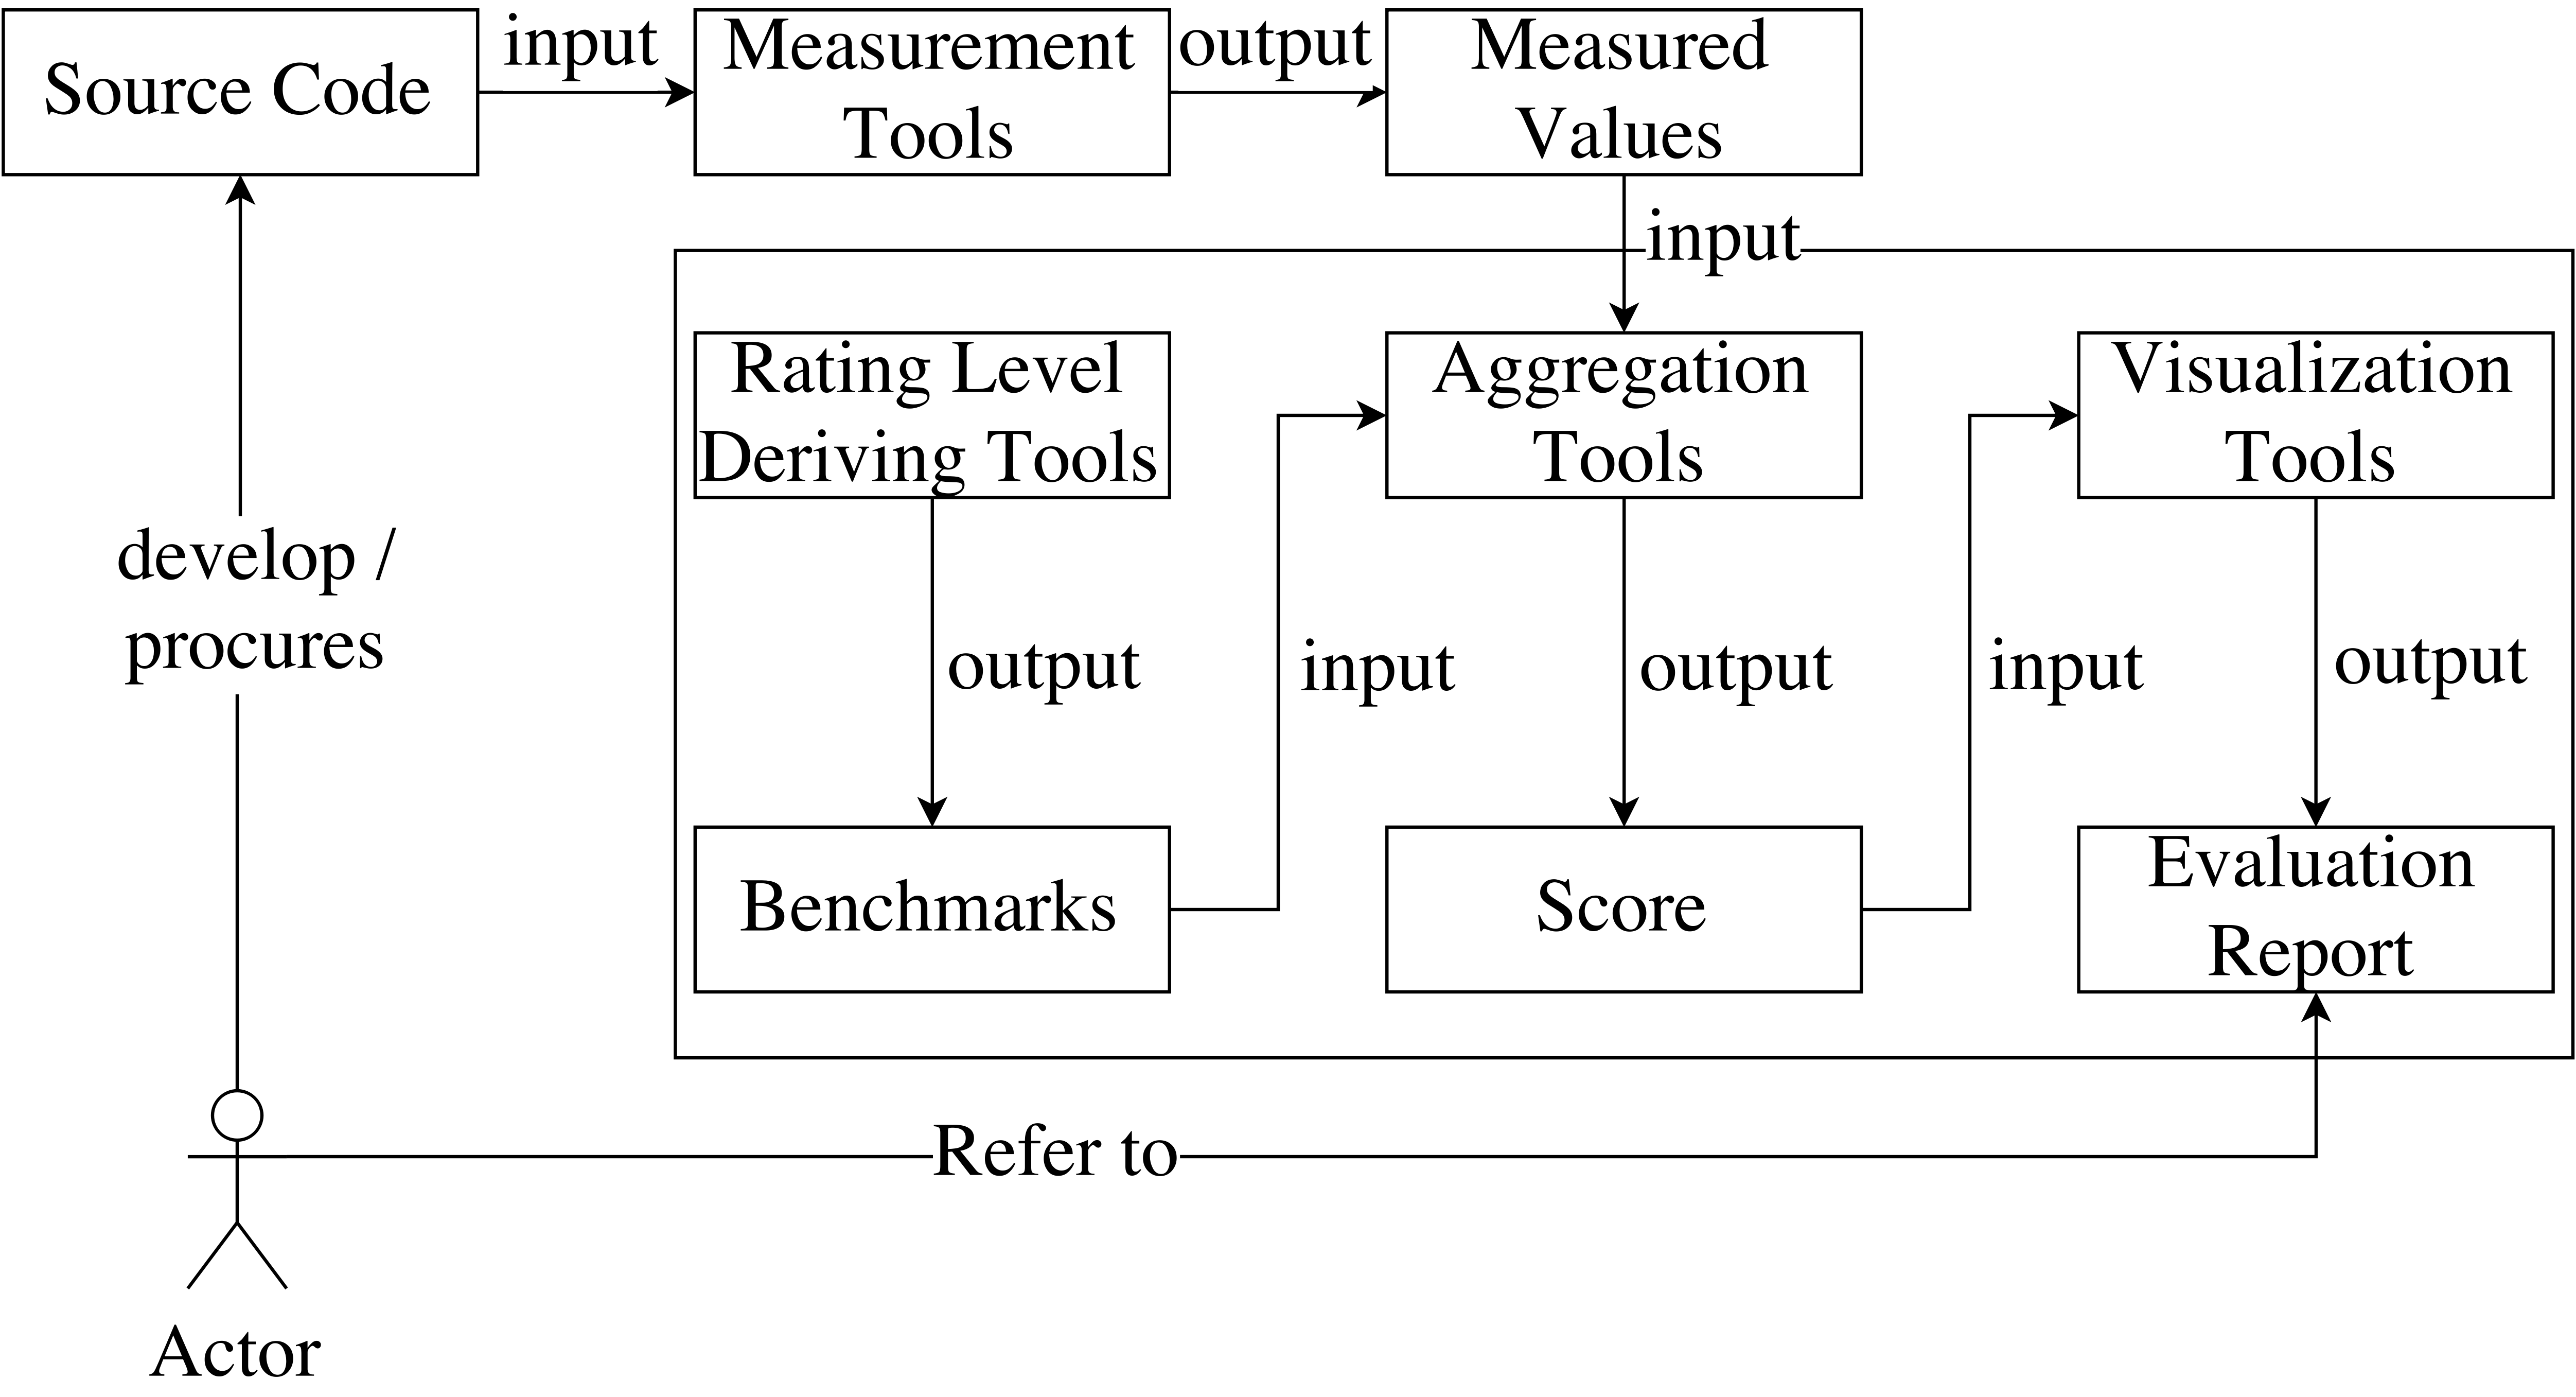
\includegraphics[width=14cm]{washizaki_framework.png}
    \caption{Structure of the quality measurement/evaluation framework derive from \cite{washizaki2007framework} paper}
    \label{figure:washizaki_framework}
\end{figure}

The core component of SQAT is highly depend on this framework, which will be mentioned in section \ref{section:architecture_of_sqat_core}. The comprehensive quality metrics suite, the technique for normalization of measured values, and the aggregation tool will be discussed in details in section \ref{section:score_calculator}. The visualisation tool will be discussed in details in section \ref{section:flux_architecture} and \ref{section:frontend_development}. 

\section{Open Source Tool: SonarQube}

In this section, we analyse a similar open source tool called SonarQube \footnote{The project is hosted on GitHub: https://github.com/SonarSource/sonarqube}. SonarQube is a continuous code inspection tool. The best way to analyse this tool is to install it and use it to analyse SQAT project. 

We used Docker to install SonarQube locally \footnote{The Docker images of SonarQube: https://hub.docker.com/\_/sonarqube/}. After the installation process, we can access the SonarQube dashboard. The SonarQube dashboard contains a welcome message, a list of projects, a list of favorite projects, and a visualisation of project metrics, as shown in Figure \ref{figure:sonar_dashboard}. We also installed SonarQube Scanner, which is the default launcher to analyze a project with SonarQube \footnote{It can be downloaded at http://bit.ly/sonarqube-runner}.

\begin{figure}[t]
    \centering
    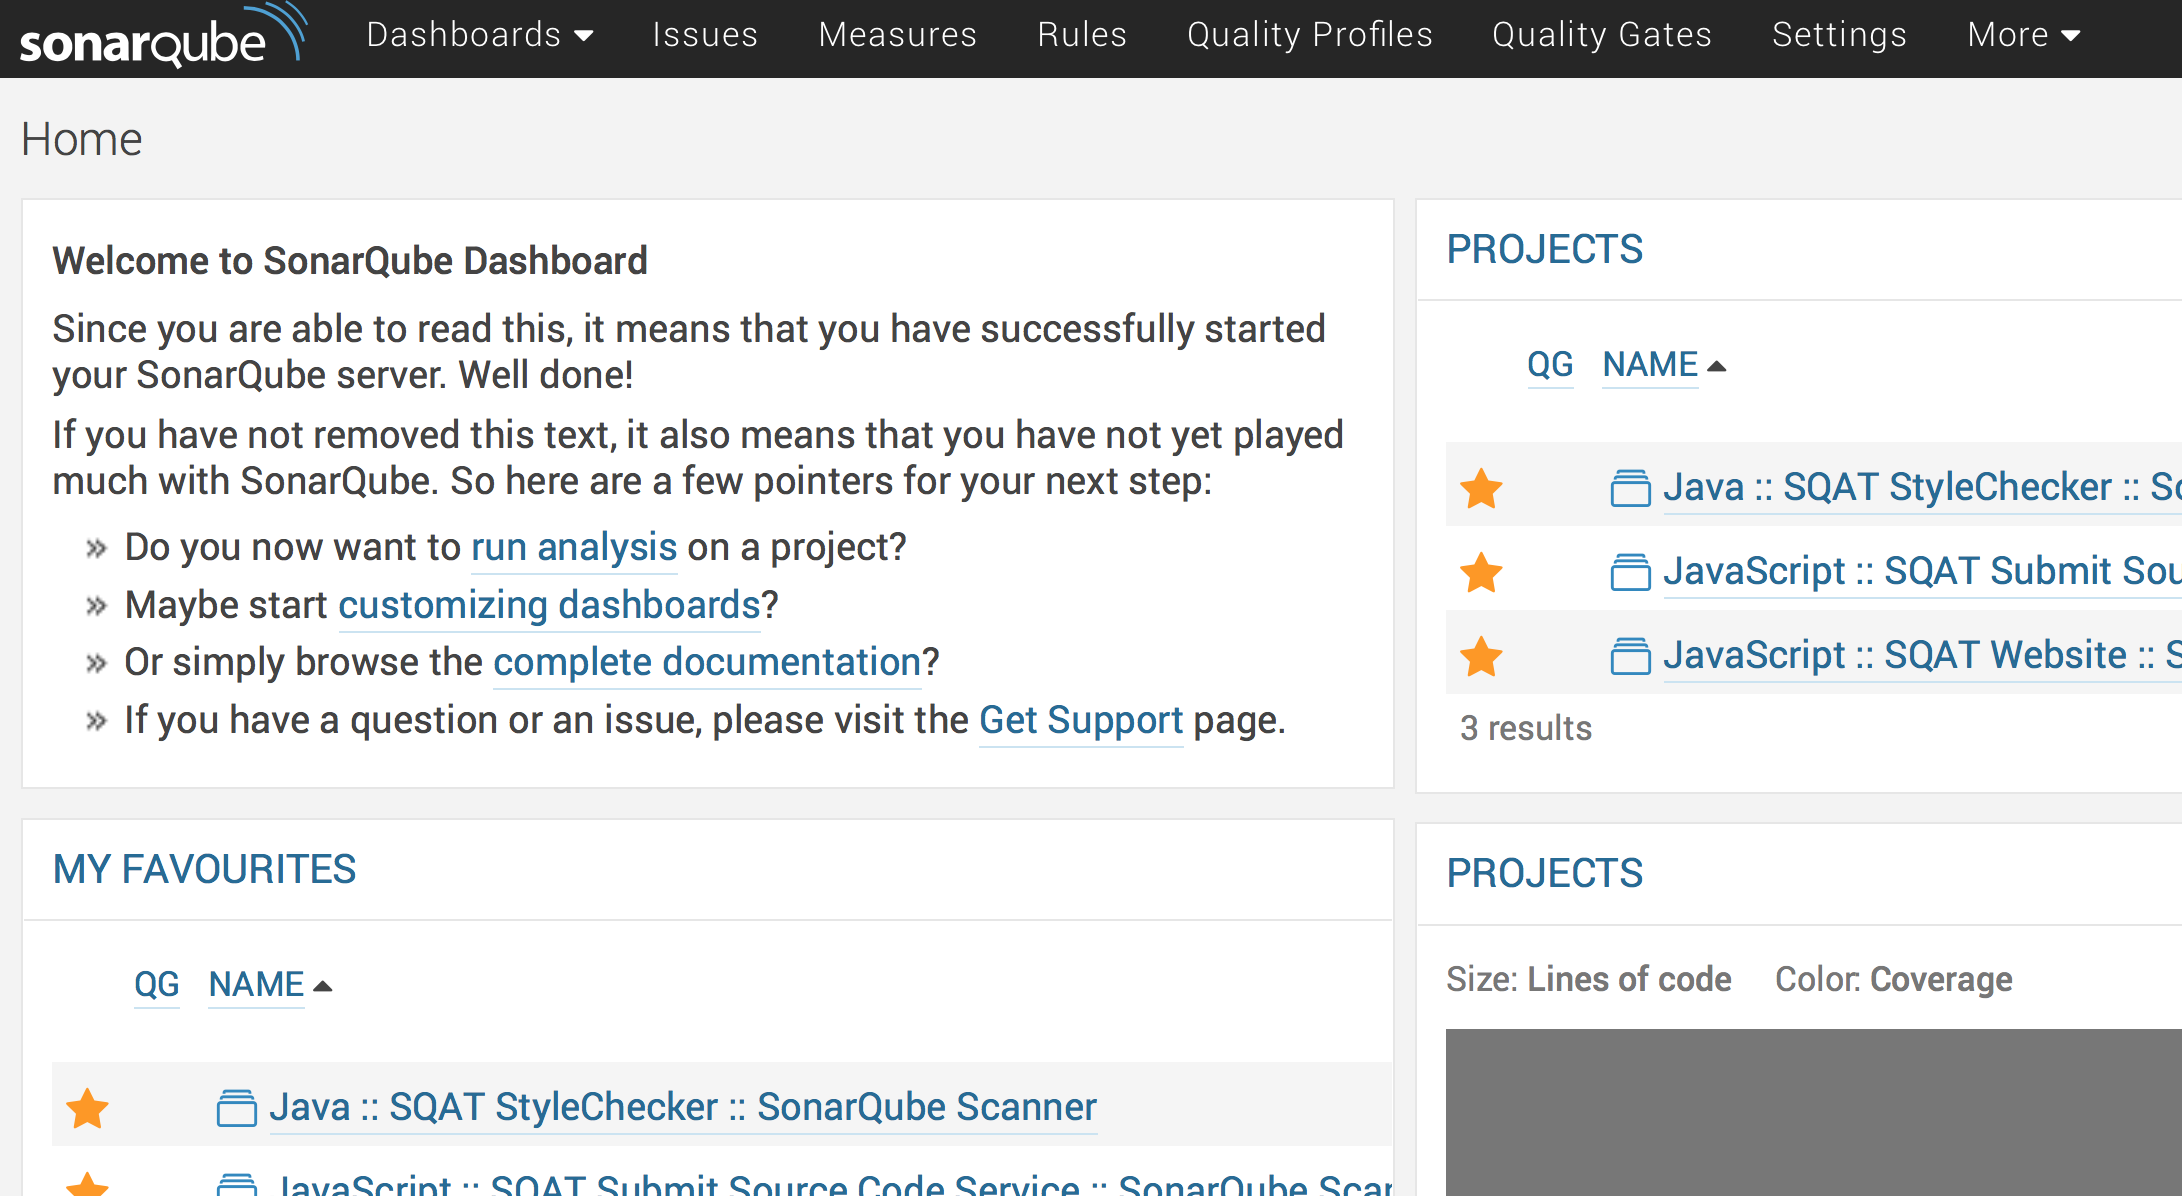
\includegraphics[width=14cm]{sonar_dashboard.png}
    \caption{Dashboard of SonarQube}
    \label{figure:sonar_dashboard}
\end{figure}

SonarQube can support more than 20 different programming languages, with various plugins, such as integration plugins, Software Configuration Management Engine, and Visualisation. Since SQAT contains Java and Javascript codes, we installed the Java and Javascript plugins. 

Next, we wrote configuration files for each component in SQAT, i.e. the main component that perform code assessment (Java), a micro-service that provide an API for client to submit request to the main component (Javascript), and a front-end component (Javascript). Configuration file for the main component is shown in Figure \ref{figure:sonarqube_config}. After all these configurations, we used the command line tool, SonarQube Runner, that we installed earlier to upload our projects to SonarQube server for assessment. 

\begin{figure}[t]
\begin{minted}
[frame=single,baselinestretch=1.0,fontsize=\footnotesize]
{python}
# Required metadata
sonar.projectKey=org.sonarqube:sqat-stylechecker
sonar.projectName=SQAT StyleChecker
sonar.projectVersion=1.0

# Comma-separated paths to directories with sources
sonar.sources=src

# Language
sonar.language=java

# Encoding of the source files
sonar.sourceEncoding=UTF-8
\end{minted}
\caption{An example of SonarQube project configuration file}
\label{figure:sonarqube_config}
\end{figure}

We now got 3 dashboards for 3 projects. The dashboard for our main component is shown in Figure \ref{figure:sonar_project_dashboard}. The first section in the dashboard shows some simple statistics, such as number of files, lines of code, directories, functions, classes, statements and accessors. The second section shows the percentage of code duplication. The third section shows the complexity of the project. The last section shows the technical dept of the project and all issues in the project. All metrics can be drilled down to a line of code and zoomed out to project level, as shown in Figure \ref{figure:sonar_project_dashboard} and Figure \ref{figure:sonar_code_issue}.

\begin{figure}
    \centering
    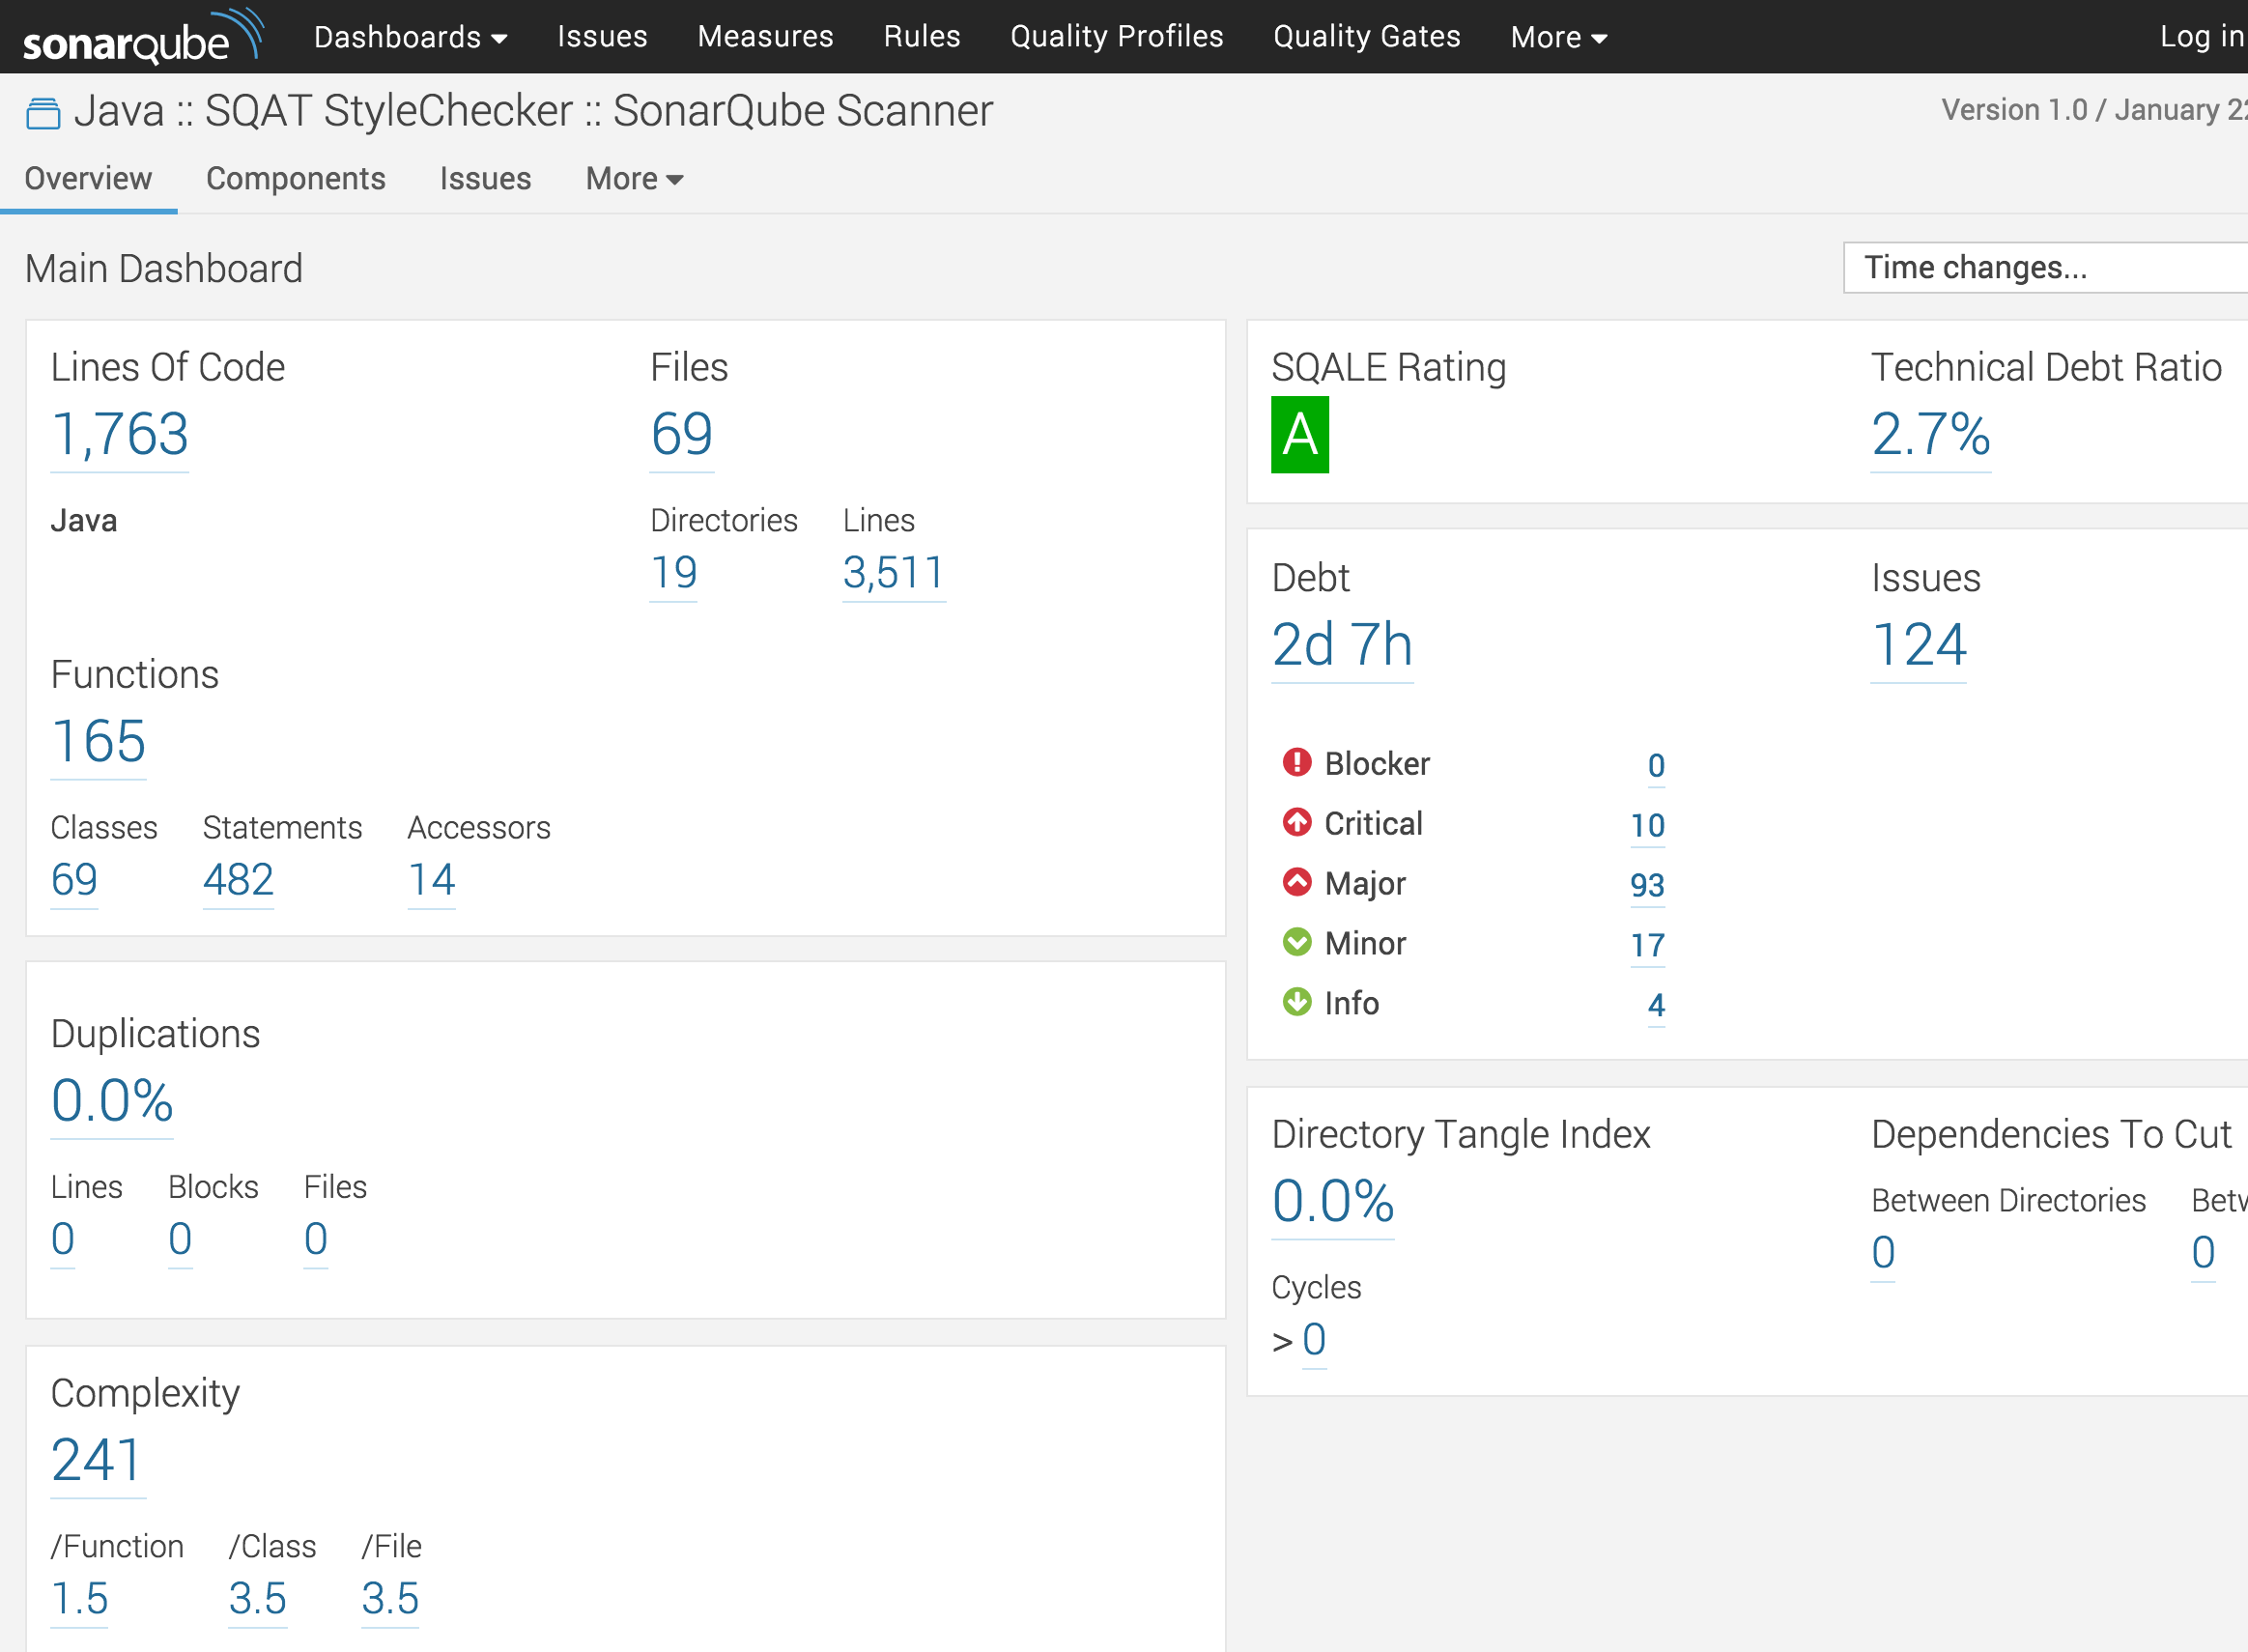
\includegraphics[width=14cm]{sonar_project_dashboard.png}
    \caption{Dashboard of a project in SonarQube}
    \label{figure:sonar_project_dashboard}
\end{figure}

\begin{figure}
    \centering
    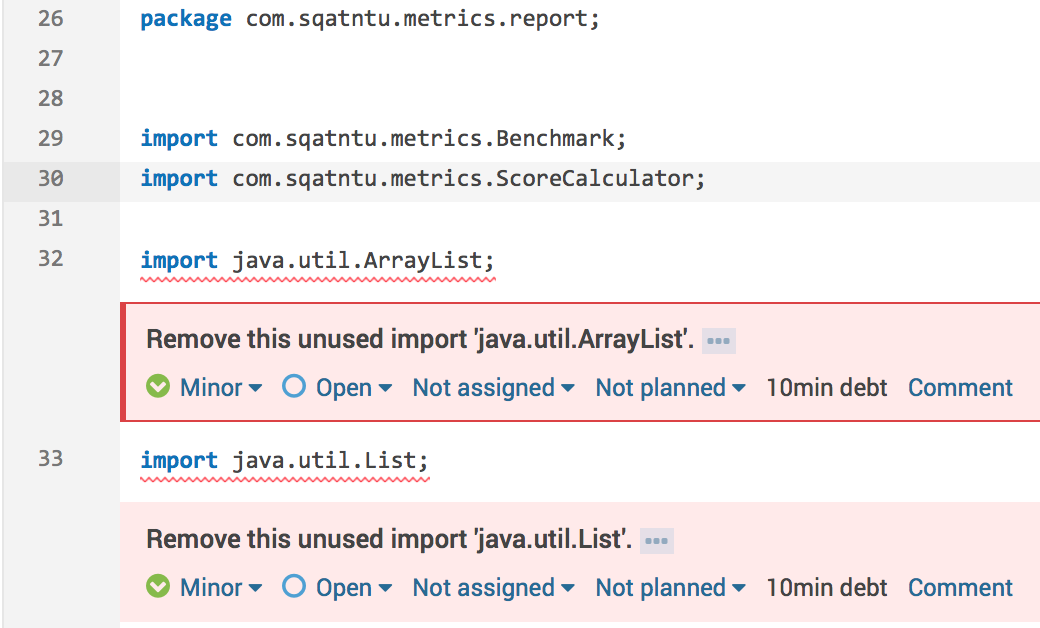
\includegraphics[width=14cm]{sonar_code_issue.png}
    \caption{Automatic code issue generated by SonarQube}
    \label{figure:sonar_code_issue}
\end{figure}

We learn 5 things when using SonarQube to analyse SQAT project. First, students and professors might want to have a dashboard so that they can view all the assignments and projects in a glance. Second, SQAT need to support different programming languages that have been used extensively in School of Computer Engineering, i.e. C, C++, Java, Python, and Matlab. Third, we need to allow students and professors to change configurations for projects and assignments because different projects and assignments have different folder organisations, programming languages, and encoding types. Fourth, SQAT must allow users to zoom out to see an overall quality of a project, and drill down to see errors in each file. Finally, line-by-line error messages and suggestion are useful for students to fix problems in their codes and improve overall code quality.

SonarQube does possess some functions we need in SQAT, such as code style checking, code duplication detection, code complexity measurements and some simple metrics. However, the goal of SonarQube project is not aligned with the goal of SQAT. The goal of SonarQube is to put technical dept under control by providing a code inspection tool. To achieve its goal, SonarQube has a great user interface for monitoring purpose. Yet, it does not provide the automation that we want in SQAT, that is, automatically assess all student source codes. To solve the problem, we probably need to develop a better application programming interface (API) for SonarQube on top of current version because SonarQube does not provide a complete API to work with plugins in SonarQube. After solving the problem, we still do not have the ability to access software qualities of source codes because SonarQube only provides a list of metrics, without any relationship to quality attributes. It does not quantify source codes using a comprehensive software quality metrics suite. For example, if a piece of source code passes all tests in SonarQube, it does not mean that the source code is maintainable, analysable, and testable. To solve the problem, we probably need to develop a SonarQube plug-in and define our Goal Question Metric (GQM) implementation in this plug-in. In conclusion, if we want to develop SQAT on top of SonarQube, we need to put two projects with different goals together, improve SonarQube API, and develop a SonarQube plug-in. Although the last two actions might be tolerable, we thought that different goals in these two projects will eventually become the major bottleneck for SQAT project. Hence, we decided to develop SQAT from scratch.

\section{Commercial Tool: SciTool}

SciTool\footnote{https://scitools.com} is an integrated development environment (IDE) with many static code analysis tools. The IDE do have a comprehensive coverage of different programming languages, such as ADA, C/C++, C\#, FOTRAN, Java, and VHDL. In addition, it also allows us to visualize our codes by generating graphs, such as UML class diagrams, control flow graph, declaration graph, and dependencies graph. Furthermore, it can collect very comprehensive list of software metrics. There are around 40 software metrics that can be collected by SciTool, as listed in their website. 

Although SciTool seems to solve some problems, but it is not what we want. We don't want to force students and professors to use a specific IDE, just because it allows us to collect software metrics and generate diagrams and graphs. In addition, SciTool has never been used by any university to assess student source codes. Their customers are usually working on commercial products, such as Dell, Ford, Adobe and BMW. Besides that, Scitool is a commercial tool that charge \$995 for one license. We believe that the management of school of computer engineering would not make commitments to an unproven solution. Furthermore, SciTool is not able to make sense of these software metrics, that is, it is not able to relate these software metrics to software qualities. As a result, SciTool is not within our consideration to achieve our objective.